\begin{figure}
\label{hists}
\centering
\subfloat[R]{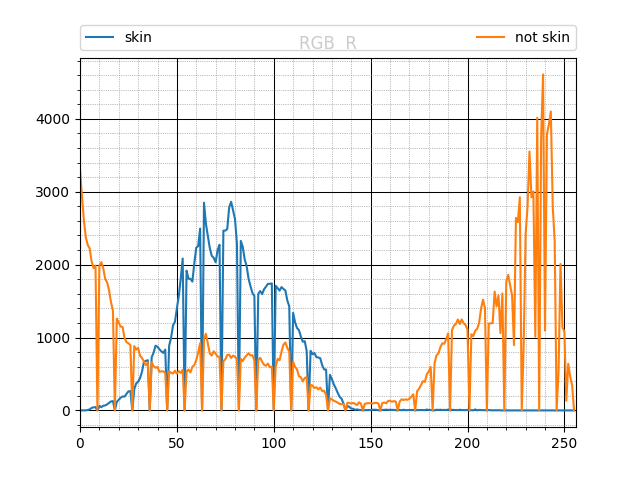
\includegraphics[width=2.6cm]{RGB-R.png}}\hfil
\subfloat[G]{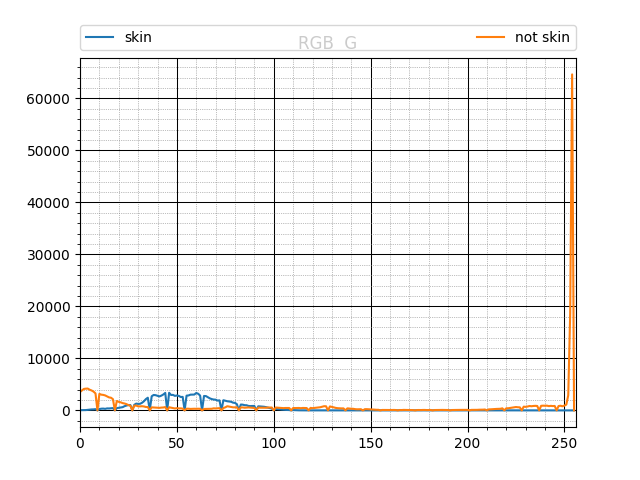
\includegraphics[width=2.6cm]{RGB-G.png}}\hfil 
\subfloat[B]{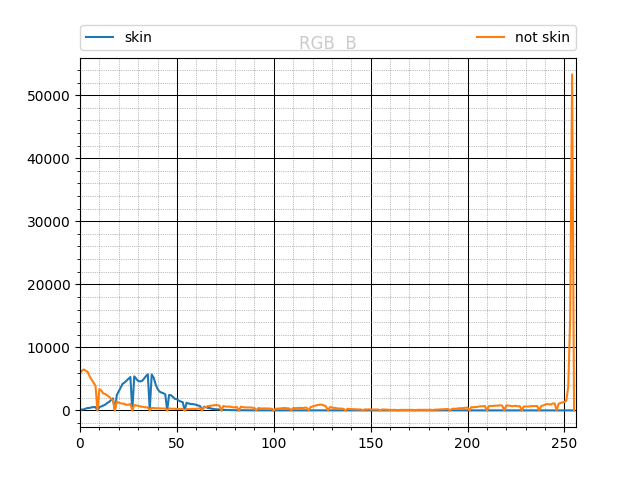
\includegraphics[width=2.6cm]{RGB-B.png}} 

\subfloat[Y]{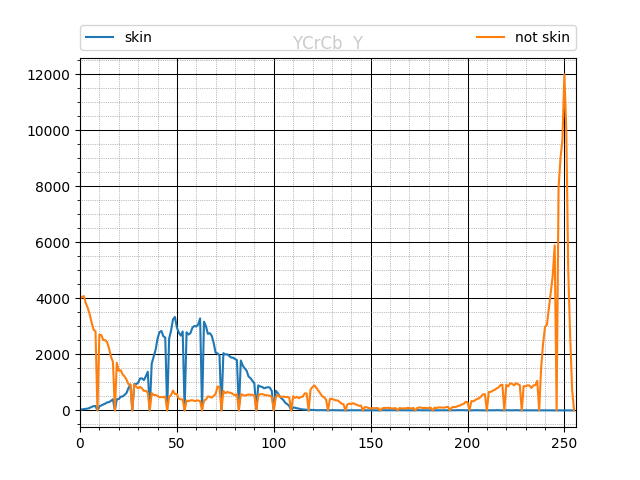
\includegraphics[width=2.6cm]{YCrCb-Y}}\hfil   
\subfloat[Cb]{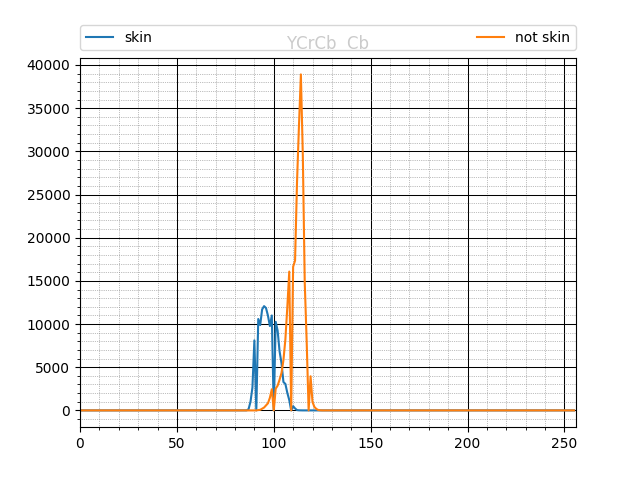
\includegraphics[width=2.6cm]{YCrCb-Cb}}\hfil
\subfloat[Cr]{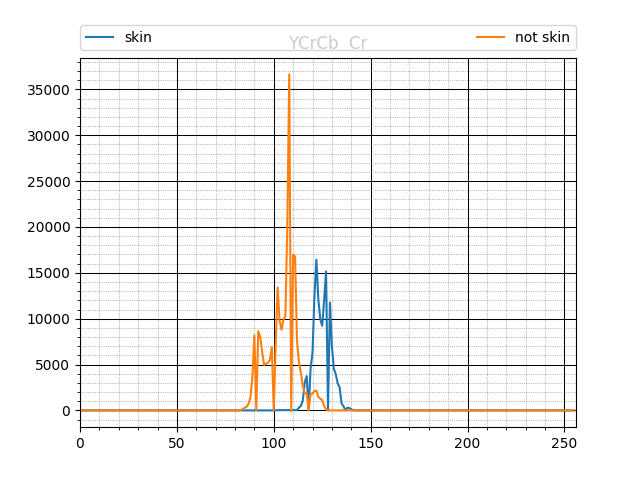
\includegraphics[width=2.6cm]{YCrCb-Cr}}
\caption{Histograma por canal dos pixels da base de treina- mento SFA reduzida}\label{figure}
\end{figure}